\section{Methodology}

\subsection{N-Dimension Matrix}
\begin{frame}
  \frametitle{N-dimension Matrix}
  \framesubtitle{Challanges}
  STL provides containers \texttt{std::array} and \texttt{std::vector} for creating one-dimension array.
  \\
  There are two way for dealing with high-dimension data:
  \begin{enumerate}
    \item Nesting the one dimension arrays or vectors.
    \item Hierarchy approach, designing derived classes of one-dimension array base class.
  \end{enumerate}
  \begin{figure}[htbp]
    \centering
    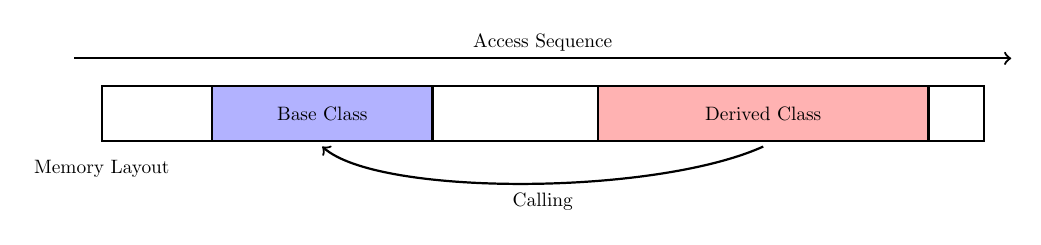
\begin{tikzpicture}[scale=0.7, transform shape]
      % \draw[help lines, step=1] (-10,-2) grid (10,2);    
      % % Draw axes
      % \draw[dashed,->] (-10,0) -- (10,0) node[right] {x};
      % \draw[dashed,->] (0,-2) -- (0,2) node[above] {y};

      \draw[thick, ->] (-8.5, 1.5) -- node[midway, above] {Access Sequence} (8.5, 1.5);

      \draw[thick] (-8,1) rectangle (8,0);
      \node at (-8,-0.5) [] {Memory Layout};

      \draw[thick, fill=blue!30] (-6,1) rectangle (-2,0);
      \node at (-4, 0.5) [] {Base Class};

      \draw[thick, fill=red!30] (1,1) rectangle (7,0);
      \node at (4, 0.5) [] {Derived Class};

      \node at (0, -1.1) [] {Calling};
      \draw[thick, ->] (4, -0.1) 
        .. controls (2, -1) and (-3, -1) .. (-4, -0.1);

    \end{tikzpicture}
    \caption{Derived Class calling members in Base class, timing is not predictable.}
    \label{<label>}
  \end{figure}
\end{frame}


\begin{frame}
  % \frametitle{N-dimension Matrix}
  % \framesubtitle{Memory Layout Problem}
  \begin{enumerate}
    \item Nesting multi-dimension array has non-contiguous memory layout.
    \item Derived class needs more time to access members in base class.
    \item Poor cache utilization leads to poor performance.
    \item MPI type create requires contiguous memory layout.
  \end{enumerate}
  % 插入图
  \begin{figure}[htbp]
    \centering
    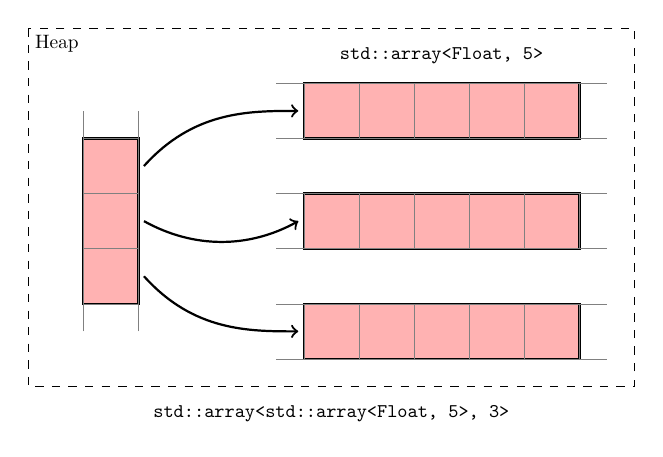
\begin{tikzpicture}[scale=0.7, transform shape]
      % \draw[help lines, step=1] (-10,-2) grid (10,2);    
      % Draw axes
      % \draw[dashed,->] (-10,0) -- (10,0) node[right] {x};
      % \draw[dashed,->] (0,-2) -- (0,2) node[above] {y};

      \draw[dashed] (-1, 3) rectangle (10, -3.5);
      \node at (-1, 3) [below right] {Heap}; 
      
      \node at (4.5, -4) [] {\texttt{std::array<std::array<Float, 5>, 3>}};
      \node at (6.5, 2.5) [] {\texttt{std::array<Float, 5>}};


      \draw[thick, fill=red!30] (0, 1) rectangle (1, -2);
      \draw[help lines, step=1] (0,1.5) grid (1,-2.5);


      \draw[thick, fill=red!30] (4, 2) rectangle (9, 1);
      \draw[help lines, step=1] (3.5, 2) grid (9.5, 1);
      
      \draw[thick, fill=red!30] (4, 0) rectangle (9, -1);
      \draw[help lines, step=1] (3.5, 0) grid (9.5, -1);
      

      \draw[thick, fill=red!30] (4, -2) rectangle (9, -3);
      \draw[help lines, step=1] (3.5,-2) grid (9.5,-3);


      \draw[thick, ->] (1.1, 0.5) 
      .. controls (2, 1.5) and (3, 1.5) .. (3.9, 1.5);

      \draw[thick, ->] (1.1, -0.5) 
      .. controls (2, -1) and (3, -1) .. (3.9, -0.5);

      \draw[thick, ->] (1.1, -1.5) 
      .. controls (2, -2.5) and (3, -2.5) .. (3.9, -2.5);
      
    \end{tikzpicture}
    \caption{Using nested \texttt{std::array<T, N>} to store 2D array data.}
    \label{<label>}
  \end{figure}
\end{frame}


\begin{frame}
  \frametitle{N-dimension Matrix}
  \framesubtitle{Solution}
  \begin{itemize}
    \item An external small \texttt{\_\_multi\_array\_shape} object defines the routines for accessing the elements.
    \item Smart pointer, ensure memory's contiguous layout and safety.
    \item Separate into two detail and user interface objects adhering RAII rules.
  \end{itemize}


  % 插入图
  \begin{figure}[htbp]
    \centering
    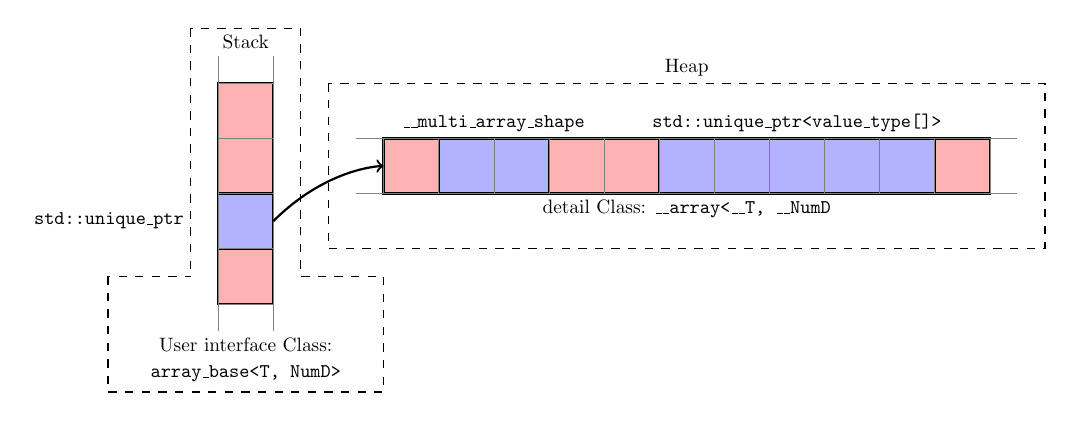
\begin{tikzpicture}[scale=0.7, transform shape]
      % \draw[help lines, step=1] (-10,-2) grid (10,2);    
      % % Draw axes
      % \draw[dashed,->] (-10,0) -- (10,0) node[right] {x};
      % \draw[dashed,->] (0,-2) -- (0,2) node[above] {y};
      
  
      \draw[dashed] (-2, 2) rectangle (11, -1);
      \node at (4.5, 2) [above] {Heap}; 

      \draw[thick, fill=red!30] (-1, 1) rectangle (10, 0);
      \node at (4.5, 0) [below] {detail Class: \texttt{\_\_array<\_\_T, \_\_NumD}};

      \draw[thick, fill=blue!30] (0, 1) rectangle (2, 0);
      \node at (1, 1) [above] {\texttt{\_\_multi\_array\_shape}};
      \draw[thick, fill=blue!30] (4, 1) rectangle (9, 0);
      \node at (6.5,1) [above] {\texttt{std::unique\_ptr<value\_type[]>}}; 
      \draw[help lines, step=1] (-1.5, 1) grid (10.5, 0);    


      
      
      \node at (-3.5, 3) [below] {Stack}; 
      \draw[dashed] (-4.5, 3) rectangle (-2.5, -3);
      \draw[dashed, fill=white] (-6, -1.5) rectangle (-1, -3.6);

      \draw[draw=none, fill=white] (-4.5, -1.9) rectangle (-2.5, -2.1);
      \draw[draw=none, fill=white] (-4.5, -1.45) rectangle (-2.5, -1.55);



      \draw[thick, fill=red!30] (-4, 2) rectangle (-3, -2);
      \draw[thick, fill=blue!30] (-4, 0) rectangle (-3, -1);
      \node at (-4.5, -0.5) [left] {\texttt{std::unique\_ptr}}; 
      \draw[help lines, step=1] (-4, 2.5) grid (-3, -2.5);    


      


      \node at (-3.5, -2.5) [below] {User interface Class:};
      \node at (-3.5, -3) [below] {\texttt{array\_base<T, NumD>}};
      \draw[thick, ->] (-3, -0.5) 
        .. controls (-2, 0.5) and (-1, 0.5) .. (-1, 0.5);

      

    \end{tikzpicture}

    \captionsetup{width=0.8\textwidth}
    \caption{
      The solution of N-dimension Matrix, using detail Class, user interface Class and a shape management structure.
    }
    \label{<label>}
  \end{figure}
\end{frame}







\subsection{Parallelization of N-dimension Arrays}
\begin{frame}
  \frametitle{Parallelization of N-dimension Arrays}
  \framesubtitle{MPI Environment}
  \hspace*{1em}The hybrid PDE solver requires the MPI supports multi-threads on each processes.\vspace*{1em}
  \begin{itemize}
    \item High-level libraries like Boost.MPI  
    \begin{enumerate}
      \item have better MPI resource management and other basic communication features.
      \item only provide limited useful features for latter PDE solvers.
      \item lead to lower performance than low-level OpenMPI. \vspace*{1em}
    \end{enumerate}
    \item I developed an environment class for MPI 
    \begin{enumerate}
      \item better resource management than raw MPI.
      \item provides basic features exclusively for this project.
    \end{enumerate}
  \end{itemize}
  
  \vspace*{1em}\hspace*{1em}

  % Creating an environment class for MPI resource management and provides basic features.

  % Ghost communication is required in overlapping of MPI communication and local computation.
  % Implementing distributions on class derived from N-dimension array class downgrades performance.

\end{frame}


\begin{frame}
  \frametitle{Parallelization of N-dimension Arrays}
  \framesubtitle{MPI Topology - Challanges}
  
  Distributed N-dimension arrays are created based on MPI N-dimension Cartesian topology.
  \begin{enumerate}
    \item Ghost communication is required in overlapping of MPI communication and local computation.
    \item Parallel I/O is needed for debugging and storing results.
    \item Topology information will be frequently used in PDE solver.
  \end{enumerate}
\end{frame}


\begin{frame}
  \frametitle{Parallelization of N-dimension Arrays}
  \framesubtitle{MPI Topology - Solution}
  \begin{enumerate}
    \item An MPI Topology class defines the distribution details of N-dimension array.
    \item Using \texttt{MPI\_Type\_create\_subarray} for creating Ghost MPI datatype for communication.
    \item Cartesian array has members Topology class and N-dimension array class, to ensure they are closely located on memory.
    \item The external functions provide gather-based I/O and MPI I/O for handling different scenarios.
    \item User interface class unified features for both topology and array classes.
    \item Separate into two detail and user interface objects adhering RAII rules.
  \end{enumerate}
\end{frame}



\section{Implementations}
\subsection{PDE Solvers}
\begin{frame}
  \frametitle{N-dimension Boundary and Initial Conditions}
  \framesubtitle{Challanges}
  \begin{enumerate}
    \item Mathematical function needs be discretized and distributed as well.
    \item Need to access the data.
    \item Initial and Dirichlet boundary conditions only applies once.
    \item Von Neumann boundary condition participates the evolving process in FDM.
  \end{enumerate}
\end{frame}


\begin{frame}
  \frametitle{N-dimension Boundary and Initial Conditions}
  \framesubtitle{Solution}
  \begin{enumerate}
    \item Use lambda function to construct classes.
    \item Creating external classes for each conditions as the friend classes of PDE solver classes.
    \item Set Bool vectors help to determine the status of conditions and type of boundary conditions.
  \end{enumerate}
\end{frame}


\begin{frame}
  \frametitle{N-dimension PDE solvers}
  \framesubtitle{Challanges}
  \begin{enumerate}
    \item 
  \end{enumerate}
  

\end{frame}

% % \subsection{General Setups}
% % \subsection{Parallel Strategies}


\subsection{PINN Model}
\begin{frame}
  \frametitle{}

  

\end{frame}
